% !TEX TS-program = XeLaTeX
%!TEX encoding = UTF-8 Unicode
%==================================================
%      PREAMBOLO e DICHIARAZIONI INIZIALI
%==================================================
\documentclass[10pt,oneside,a4paper]{article}

\usepackage[utf8]{inputenc} 
\usepackage[italian]{babel}
\usepackage[T1]{fontenc}
\usepackage{siunitx} %Inserisce automaticamente i dati con le unità  di misura correttamente formattate del SI (utilizzo: \SI{0.82}{m^2}, in generale \SI{misura con il punto decimale}{unità  di misura})
\sisetup{output-decimal-marker = {.}, separate-uncertainty = true, input-uncertainty-signs = \pm, detect-weight=true, detect-family=true} %per usare SI con il punto decimale
\usepackage{listings} %Per citare codice informatico formattandolo correttamente
\usepackage{amsmath,amsthm,verbatim,amssymb,amsfonts,amscd,graphicx,mathtools}
\usepackage[makeroom]{cancel}
\newcommand{\abs}[1]{\left\lvert\,#1\,\right\rvert}
\usepackage{geometry}
\usepackage{epigraph}
\usepackage{booktabs}	%tabelle migliorate
\usepackage{tablefootnote}	%note a piè di pagina in tabella
\usepackage{threeparttable} %tabella con note a piè di tabella
\usepackage{caption}	%descrizione per figure
\usepackage{dblfnote}
\usepackage{supertabular}
\usepackage{longtable}
\captionsetup{tableposition=top,figureposition=bottom,font=small} %setup descrizione
\usepackage{float}
\usepackage{esvect} %vettori
\usepackage{longtable} %tabelle lunghe
\usepackage[dvipsnames]{xcolor}
\definecolor{sepia}{HTML}{80002A}
\usepackage[colorlinks=true, citecolor=black, linkcolor=sepia, urlcolor=black]{hyperref}
\usepackage{mathrsfs}
\usepackage{circuitikz}
\tikzset{
  font={\fontsize{7pt}{12}\selectfont}}
\ctikzset{bipoles/resistor/height=0.2}
\ctikzset{bipoles/resistor/width=0.4}
\ctikzset{bipoles/diode/height=0.3}
\ctikzset{bipoles/diode/width=0.3}
\ctikzset{tripoles/american nand port/height=0.7}
\ctikzset{tripoles/american nand port/width=0.8}
\usepackage{enumitem} %Liste senza spazi verticali
\setlist{noitemsep}
\usepackage{amsmath}
\usepackage{hyperref}
%\usepackage{pst-optexp} %Diagrammi ottici
\usepackage{physics} %Ambienti utili
\usepackage{upgreek} %Per avere lettere greche non corsive, ex. \upbeta


\interfootnotelinepenalty=10000


\usepackage{multicol}
\newenvironment{Figure}
  {\par\medskip\noindent\minipage{\linewidth}}
  {\endminipage\par\medskip}

%\newcommand{\var}{\operatorname{var}}
%\newcommand{\cov}{\operatorname{cov}}


\usepackage{listings} %Per inserire codice
\lstdefinestyle{CStyle}{
    backgroundcolor=\color{backgroundColour},   
    commentstyle=\color{mGreen},
    keywordstyle=\color{magenta},
    numberstyle=\tiny\color{mGray},
    stringstyle=\color{mPurple},
    basicstyle=\footnotesize\ttfamily,
    breakatwhitespace=false,         
    breaklines=true,                 
    captionpos=b,                    
    keepspaces=true,                 
    numbers=left,                    
    numbersep=5pt,                  
    showspaces=false,                
    showstringspaces=false,
    showtabs=false,                  
    tabsize=2,
    language=C
}

\definecolor{color1}{RGB}{90,0,0} % Color of the article title and sections
\definecolor{color2}{RGB}{0,20,50} % Color of the boxes behind the abstract and headings
\definecolor{mGreen}{rgb}{0,0.6,0}
\definecolor{mGray}{rgb}{0.5,0.5,0.5}
\definecolor{mPurple}{rgb}{0.58,0,0.82}
\definecolor{backgroundColour}{rgb}{0.95,0.95,0.92}


%==================================================
%                  PRIMA PAGINA
%==================================================

\title{\textsc{\textbf{Esperienza 5}: Lamine di ritardo e misura dei parametri di Stokes}}
\author{\small{G. Galbato Muscio} \and \small{F. Ghimenti} \and \small{L. Gravina} \and \small{L. Graziotto}}
\date{30 Maggio 2019}

\begin{document}
	\begin{figure}
		\centering
		\includegraphics[scale=0.5, trim={2.8cm 8.9cm 0 9cm}, clip]{logo.png}
	\end{figure}
	\maketitle
	\begin{center} 
		\fbox{{\fontsize{12pt}{8mm}\textsc{Gruppo D1-1}}} \\
	\end{center}
\hrule
\vfill
\renewcommand{\abstractname}{Abstract}
\begin{abstract}
Si individuano gli assi principali di due lamine di ritardo rispettivamente a $\lambda/2$ e a $\lambda/4$, quindi si controlla la bontà della taratura della $\lambda/4$. Avendo a disposizione le inclinazioni degli assi principali, si usano le lamine per misurare i parametri di Stokes di un fascio uscente da un \emph{beam splitter} polarizzatore e del fascio laser originale; infine, usando un filtro polaroid e una seconda lamina a $\lambda/4$ si mappa la sfera di Poincaré. 
\end{abstract}
\vfill
\tableofcontents %Indice
\newpage


\pagebreak


\begin{multicols}{2}
%==================================================
%             APPARATO STRUMENTALE
%==================================================
\section{Apparato strumentale}

Si utilizza un laser He-Ne di lunghezza d'onda, dichiarata dal costruttore, $\lambda = \SI{632.8}{nm}$, montato su tavolo ottico\footnote{Si confronterà dunque il risultato sperimentale ottenuto in seguito con questo valore.}. 

In serie al laser è posta un'iride, allo scopo di evitare l'ingresso nel laser dei fasci di ritorno, che ne perturberebbero il comportamento. Due specchi orientati a \SI{45}{\degree} portano il fascio ad incidere su una sequenza di strumenti formata da \emph{beam splitter} polarizzatori e lamine di ritardo a $\lambda/4$ e $\lambda/2$, sequenza che cambia in base alla parte dell'esperienza che si sta realizzando e che quindi viene descritta all'inizio di ogni paragrafo.

Il fascio in uscita dalla sequenza di strumenti ottici è quindi portato ad incidere su un fotomoltiplicatore, con cui se ne misura l'intensità.
%\begin{Figure}
%	\begin{center}
%	\hbox{\hspace{-0.8cm}
%	\includegraphics[width=1.1\linewidth]{diagram.png}}
%	\captionof{figure}{Configurazione utilizzata.}
%	\label{fig:diagram}
%	\end{center}
%\end{Figure}
Le misure di intensità luminosa vengono riportate come differenza di potenziale misurata ai capi del fotodiodo, pertanto è da intendere la presenza di un fattore di proporzionalità non noto. Inoltre, si regola con un filtro attenuatore l'intensità della luce emessa dal laser in modo da restare all'interno della regione di linearità del fotodiodo, ossia al di sotto di \SI{10}{V}. 

In generale, tutte le misure di intensità saranno affette da un errore che è stato stimato dall'intervallo di oscillazione del voltmetro durante la misura.


%==================================================
%             TARATURA DELLE LAMINE DI RITARDO
%==================================================
\section{Taratura delle lamine di ritardo}
Si utilizza un beam splitter polarizzatore per ottenere una luce polarizzata orizzontalmente (linearmente, in un piano parallelo al piano del tavolo ottico), questa viene fatta passare attraverso una lamina di ritardo a $\lambda/2$ montata su una ghiera graduata che permette di controllarne la rotazione; il fascio in uscita dalla lamina viene fatto passare in un secondo beam splitter che ne seleziona la sola componente orizzontale, infine l'intensità di questo fascio viene misurata con il fotodiodo. Le misure sono state fatte dopo aver controllato la bontà dell'allineamento dei fasci.

Si vuole trovare l'angolo $\theta_0$ della ghiera che corrisponde ad una situazione in cui l'asse principale della $\lambda/2$ è orizzontale.

In Figura \ref{fig:taratura_lambda2} è riportato l'andamento dell'intensità misurata al variare dell'angolo di rotazione della $\lambda/2$, mentre le misure sono riportate in Tabella \ref{tab:taratura_lambda2}. Ai punti sperimentali è sovrapposto un fit dell'andamento teorico dato da
\begin{equation}
	I(\theta) = I_0 \cos^2\left( 2\left(\theta- \theta_0\right)\right)
\end{equation}
dove i parametri che meglio descrivono le misure sono $I_0 = \SI{4.48 \pm 0.05}{V}$ e $\theta_0 = \SI{0.680\pm0.005}{rad}$.
\begin{Figure}
	\begin{center}
	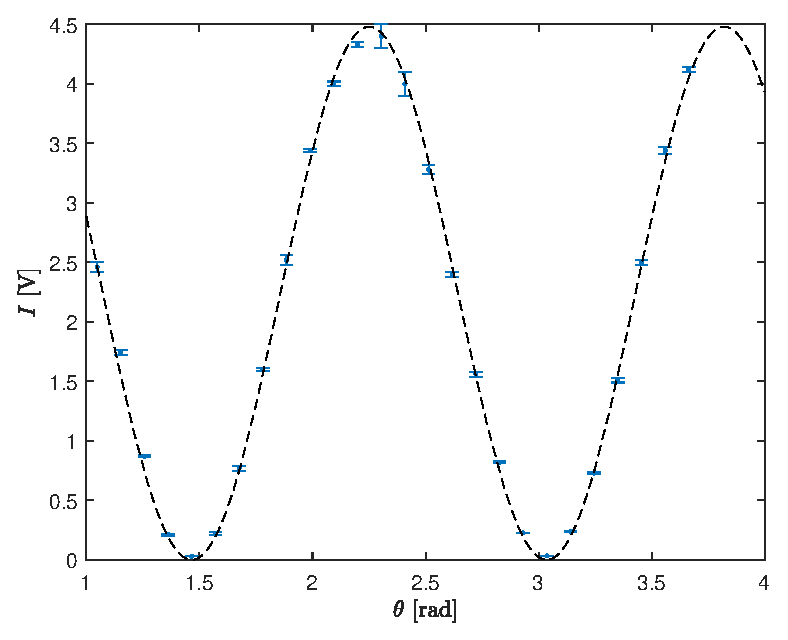
\includegraphics[width=\linewidth]{taratura_lambda2.eps}
	\captionof{figure}{Andamento della tensione misurata dal fotodiodo al variare dell'angolo di rotazione della lamina $\lambda/2$, ai dati è sovrapposto il fit del modello teorico}
	\label{fig:taratura_lambda2}
	\end{center}
\end{Figure}

Valutato l'angolo $\theta_0$ corrispondente all'asse principale della $\lambda/2$, si passa a valutare lo stesso angolo $\xi_0$ per la $\lambda/4$: quest'ultima viene montata tra il primo beam splitter e la $\lambda/2$, avendo posizionato la seconda lamina di ritardo nella configurazione per cui l'asse è orizzontale, si ruota la ghiera della $\lambda/4$ e si ottengono le misure riportate in Tabella \ref{tab:taratura_lambda4} e in Figura \ref{fig:taratura_lambda4}, in quest'ultima è anche riportato il fit del modello teorico dato da
\begin{equation}
	I(\xi) = \frac{\tilde{I}_0}{2}\left( 1- \cos^2\left(2\left(\xi-\xi_0\right)\right)\right)
\end{equation}
dove i parametri del fit che meglio descrivono le misure sono $\tilde{I}_0 = \SI{7.6\pm0.1}{V}$ e $\xi_0 = \SI{0.19\pm0.02}{rad}$.
\begin{Figure}
	\begin{center}
	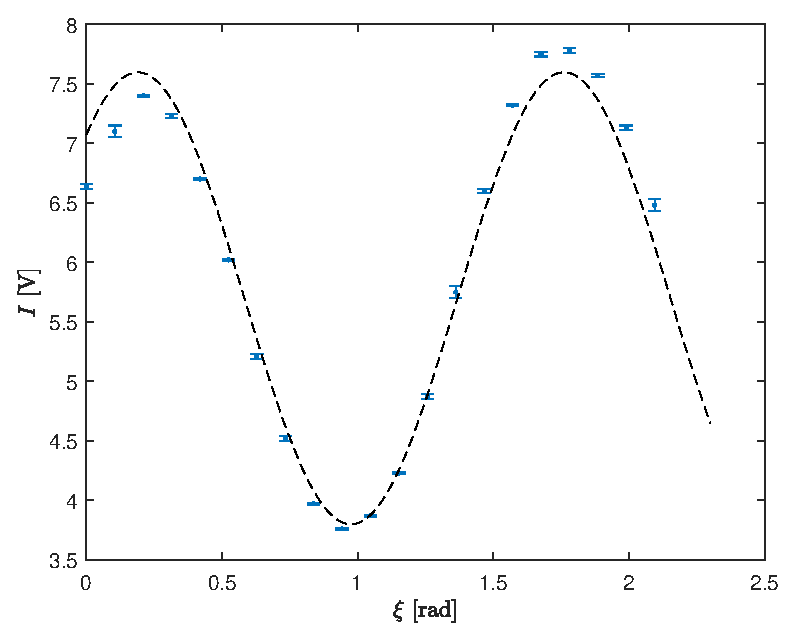
\includegraphics[width=\linewidth]{taratura_lambda4.eps}
	\captionof{figure}{Andamento della tensione misurata dal fotodiodo al variare dell'angolo di rotazione della lamina $\lambda/4$, ai dati è sovrapposto il fit del modello teorico}
	\label{fig:taratura_lambda4}
	\end{center}
\end{Figure}
Il motivo per cui si è scritto $\tilde{I}_0$ invece di $I_0$ è che nel caso ideale queste due quantità dovrebbero coincidere, ma nella nostra esperienza tra la taratura di $\lambda/2$ e quella di $\lambda/4$ sono state effettuate delle importanti operazioni di allienamento del sistema, che hanno comportato anche una modifica all'intensità massima del fascio.

Infine, si vede che la bontà del fit della taratura della $\lambda/4$ è peggiore rispetto a quello della $\lambda/2$, in particolare si confronta un coefficiente $R^2 = 0.998$ per la $\lambda/2$ con $R^2 = 0.976$ per la $\lambda/4$, si conclude che ciò è dovuto al fatto che la $\lambda/4$ è molto più sensibile a imprecisioni nell'allineamento rispetto alla $\lambda/2$.


%==================================================
%             VERIFICA DELLA BONTA' DELLA TARATURA
%==================================================
\section{Verifica della bontà della taratura della lamina a $\lambda/4$}

%==================================================
%             MISURA DEI PARAMETRI DI STOKES
%==================================================
\section{Misura dei parametri di Stokes}
\subsection{Fascio polarizzato linearmente} %Potete anche pensare di usare \paragraph invece di \subsection
\subsection{Fascio laser originale}
\subsection{Mappatura della sfera di Poincaré}


%==================================================
%             CONCLUSIONI
%==================================================
\section{Conclusioni}


\end{multicols}


\newpage
\section{Appendice}



%ESEMPIO DI FIGURA
%\begin{Figure}
%	\begin{center}
%	\includegraphics[width=\linewidth]{comune.png}
%	\captionof{figure}{Istantanea dell'oscilloscopio per l'amplificatore differenziale, misura di $A_c$}
%	\label{fig:Ac_differenziale}
%	\end{center}
%\end{Figure}


%ESEMPIO DI TABELLA
%\begin{center}
%\captionof{table}{Misure per la stima di $A_c$}
%\label{tab:Ac_differenziale}
%\begin{tabular}{c|c|c|c}
%$f$ [\SI{}{Hz}] & $V_i$ [\SI{}{V}] & $v_o$ [\SI{}{mV}] & $A_c = v_o / V_i$ \\
%\hline
%      149.5 &        3.90 &         11.3 & 2.90e-03 \\
%      222.0 &        3.90 &         11.5 & 2.95e-03 \\
%      281.0 &        3.90 &         11.8 & 3.03e-03 \\
%      359.0 &        3.90 &         11.8 & 3.03e-03 \\
%      461.0 &        3.90 &         12.2 & 3.13e-03 \\
%\hline
%\end{tabular}
%\end{center}

\end{document}
